\chapter{Análise dos Dados}\label{chapter5}
%TODO: statistical analysis, filtres(?). char, main/afeter shocks, histograms
%pesquisar alguma coisa sobre dados e GA só pra formular uma intro
\section{Dados de sismos}
O foco dessa pesquisa é estudar padrões existentes nas ocorrências de sismos. Para isso é essencial que tenhamos acesso a dados confiáveis, seguros e ricos em detalhes. Pela página da {\it Japan Metereological Agency} fomos capazes de acessar dados fiéis aos nossos interesses. Os dados obtidos são compostos por longitude, latitude, data e horário da ocorrência, magnitude e profundidade. \\
%- JMA\footnote[2]{\url {http://www.jma.go.jp/jma/index.html}}

Para a base de treino, foram separados os sismos considerados mais uniformes, formando o grupo cuja latitude e longitude na superfície representam abalos em áreas terrestres (terremotos), pouco profundos (acima de 20 km de profundidade) e com magnitude acima de 2.5 grau na escala Richter, durante os anos de 2000 a 2013.\\

Para selecionar terremotos, foi preciso extrapolar as informações contidas nos dados e buscar uma forma de, a partir dos dados disponíveis, deduzir quais sismos serão considerados terremotos e quais serão considerados maremotos. Para isso foi utilizamos {\it The Google Elevation API}\footnote[3]{\url {https://developers.google.com/maps/documentation/elevation/?hl=pt-es}}, uma {\it Application Programming Interface} (API) que tem como objetivo fornecer informações sobre todos os locais sobre a superfície terrestre e oceânica. \\

A API foi utilizada por oferecer uma interface HTTP para consulta de dados de elevação territorial, que recebe via url os parâmetros latitude e longitude e retorna, em formato {\it JavaScript Object Notation} (JSON), dados como a altitude relativa à coordenadas fornecidas, dado este necessário para nossos estudos. Os abalos cuja coordenadas na superfície terrestre tivessem altitude relativa ao nível do mar acima de 0.0 foram selecionados.\\

Ao analisar a nova base de treino percebe-se um elevado aumento na quantidade de terremotos em 2011, ano que o terremoto de Tohoku, magnitude 9 na escala Ritcher, ocorreu, Figura \ref{ocorrenciasAno}. Esse terremoto causou aumento desproporcional de sismos em todo o Japão, fato que levou a decisão de limitar a base de treino até o ano de 2010.\\

%pq???
Ainda em relação a base de treino, ela foi alterada para gerar fatias anuais da base de treino anterior, baseadas nos dados cronológicos disponíveis nos dados da JMA. As fatias são definidas da seguinte forma: se a base refere-se a sismos ocorridos em um espaço de 10 anos, a base será divida por 10, gerando fatias anuais (por exemplo, de 2004 até 2005). Dessa forma, espera-se minimizar o {\it overfitting} (super ajustes) a base de dados.\\

{\it Overfitting} é o uso de modelos ou procedimentos que violam parcimônia, isto é, que incluem mais termos que o necessário ou usam abordagens mais complicadas do que necessárias \cite{hawkins2004problem}. Visar minimiza-lo, na aplicação GA, é importante para que tenhamos boas generalizações.\\

Outra limitação imposta a base de dados foi em relação a área analisada. Como buscamos entender os padrões dos sismos, escolhemos quatro regiões do Japão para focar o experimento, Kanto, Kansai, Touhoku e East Japan. A Figura \ref{alljapan} propõe uma visualização dessas regiões no Japão. A seguir descreveremos as quatro regiões.\\

\paragraph{Kanto} Kanto é a região ao redor de Tóquio. É uma área com elevada atividade sísmica durante o período estudado. Essa região foi definida com coordenadas começando em 34.8 Norte, 138.8 Oeste, com  2025 {\it bins}. Cada {\it bin} corresponde a uma área de 25km2.\\

\paragraph{Kansai} Kansai é a região que inclui cidades Kyoto, Osaka e outras. Essa área, ao contrário da região de Kanto, possui uma baixa atividade sísmica. Essa região foi definida com coordenadas começando em 34 Norte, 134.5 Oeste, com  1600 {\it bins}. Cada {\it bin} corresponde a uma área de 25km2.\\

\paragraph{Touhoku} Touhoku é a região definida como a região ao norte da ilha principal japonesa. Ela possui alguns {\it clusters} de atividade sísmicas durante o período estudado. Essa região foi definida com coordenadas começando em 37.8 Norte, 139.8 Oeste, com  800 {\it bins}. Cada {\it bin} corresponde a uma área de 100km2. \\

\paragraph{Leste do Japão} É a região corresponde a costa leste do Japão. Ela se diferencia da área anterior por incluir tanto áreas terrestres como não-terrestres. Foi nessa área que o sismo M9 de 2011 aconteceu. Essa região foi definida com coordenadas começando em 37 Norte, 140 Oeste, com  1600 {\it bins}. Cada {\it bin} corresponde a uma área de 100km2. \\

%\begin{figure}[!htb]
%\centering
%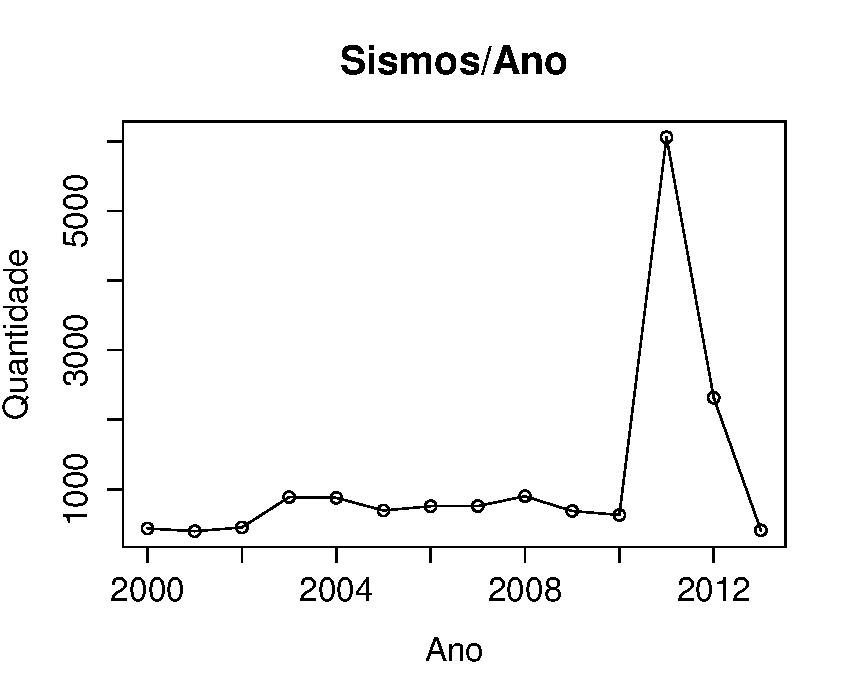
\includegraphics[scale=0.9]{ocorrenciasAno}
%\caption{Quantidade de sismos pelos anos.}
%\label{ocorrenciasAno}
%\end{figure}
%
%\begin{figure}[!htb]
%\centering
%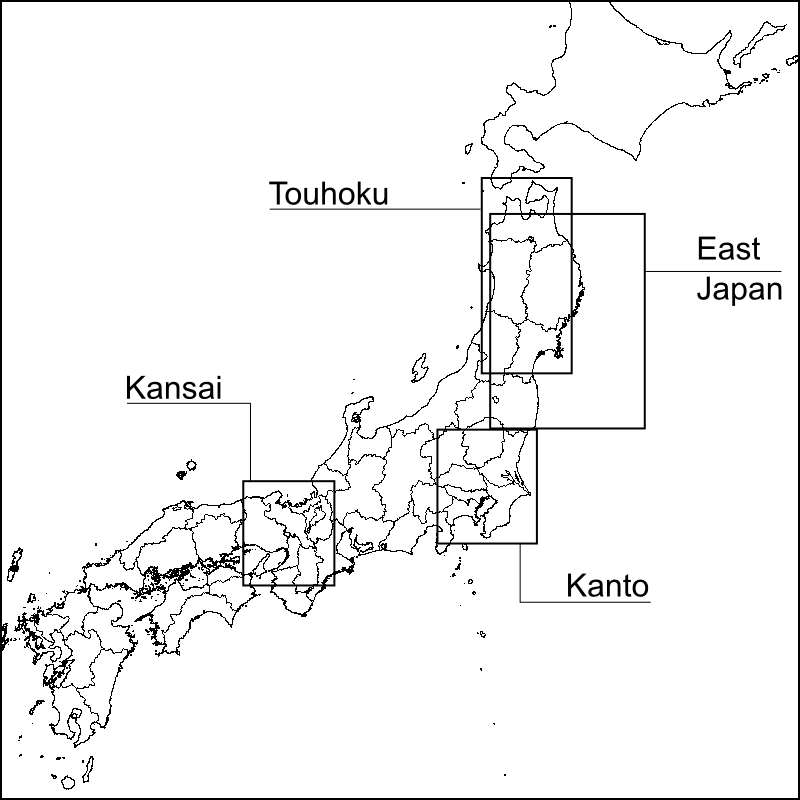
\includegraphics[scale=0.5]{alljapan.png}
%\caption{Áreas priorizadas e suas localização.}
%\label{alljapan}
%\end{figure}



%A última, se refere diretamente a nova base de treino. Ao analizar

1'